% JuliaCon proceedings template
\documentclass{juliacon}
\setcounter{page}{1}

\usepackage{amsmath}
\usepackage{tikz}

\lstdefinelanguage{Julia}%
  {morekeywords={abstract,break,case,catch,const,continue,do,else,elseif,%
      end,export,false,for,function,immutable,import,importall,if,in,%
      macro,module,otherwise,quote,return,struct,switch,true,try,typealias,%
      using,while},%
   sensitive=true,%
   alsoother={\$},%
   morecomment=[l]\#,%
   morecomment=[n]{\#=}{=\#},%
   morestring=[s]{"}{"},%
   morestring=[m]{'}{'},%
}[keywords,comments,strings]%


\lstset{
    language = Julia,
    frame = single
}

\begin{document}

% **************GENERATED FILE, DO NOT EDIT**************

\title{ModelingToolkit.jl: An Intermediate Representation for Scientific Domain-Specific Languages}

\author[1]{Harrison Grodin}
\author[2]{Yingbo Ma}
\author[3]{Christopher Rackauckas}
\affil[1]{School of Computer Science, Carnegie Mellon University}
\affil[2]{Department of Mathematics, University of California Irvine}
\affil[3]{Department of Mathematics, Massachusetts Institute of Technology}

\keywords{Julia, symbolic computation, differential equations, pharmacometrics}

\maketitle

\begin{abstract}

Domain-specific languages (DSLs) enable scientific programmers to describe their models in a high-level format while still allowing for internal optimizations. However, while the homoiconicity of Julia has encouraged the proliferation of DSLs, code reuse between DSLs has been stymied due to the lack of a common intermediate representation for performing inspection, symbolic transformation, and compilation of scientific models. In this paper, we present ModelingToolkit.jl, a Julia library and intermediate representation for scientific DSLs. We discuss the internal representations of symbolic expressions and systems, chosen to implicitly enforce logical invariants. We showcase how ModelingToolkit is being used in the pharmacometric modeling DSL Pumas.jl, and describe future improvements to incorporate this system into other Julia packages.

\headingtable

\end{abstract}

\section{Introduction}

In many applications, scientists and engineers need to perform symbolic transformations on their models in order to have a formulation that is efficiently computable by numerical methods. For example, Modelica \cite{mattsson_modelica_1997} is a language for describing physical differential-algebraic equations (DAEs) and utilizes the Pantelides algorithm \cite{doi:10.1137/0909014} to transform higher index systems to index 1 DAEs, which can be handled by numerical solvers like DASSL \cite{petzold_description_nodate} or the IDA method of SUNDIALS \cite{alan_c._hindmarsh_sundials:_2005}. NONMEM \cite{sheiner1977estimation} is a domain-specific language for pharmacometrics in Fortran that reads a text file describing differential equation models and appends the sensitivity equations utilized by parameter estimation routines. These packages are just two among many which have developed their own internal systems for performing the steps necessary to handle this process, which includes:

\begin{itemize}
    \item Parsing a text file into an internal representation (IR).
    \item Performing transformations on the IR to build new model expressions.
    \item Compiling the expressions to a common format to be utilized by numerical methods.
\end{itemize}

While the distinct tools achieve the goals of the end user, the internal mathematical systems for computing the model transformations cannot be utilized outside of their respective frameworks.

The Julia programming language \cite{bezanson_julia:_2017} is a high-level dynamic language for scientific computing which is able to generate compiled code with performance on par with C and Fortran. Julia is notably homoiconic, with macros that allow users to manipulate Julia expressions without writing a custom parser. This abstraction greatly simplifies the construction of domain-specific languages (DSLs) which has led to the proliferation of DSLs throughout the Julia package ecosystem. For example, the differential equation solvers of DifferentialEquations.jl \cite{christopher_rackauckas_differentialequations.jl_2017} has an {\verb @ode_def } macro which converts simple differential equation expressions into Julia functions usable by numerical methods. DiffEqBiological.jl \cite{diffeqbiological} includes the {\verb @reaction_network } DSL that describes a system of chemical reactions and creates Julia functions for the ordinary differential equation, stochastic differential equation, and jump equation solvers. An example of the reaction network DSL is shown in Figure \ref{code:reaction}, taking in a description of the reactions and generating the chemical kinetics expressions corresponding to the included system.

\begin{figure}
\begin{subfigure}%[h]{0.45\textwidth}
\begin{lstlisting}
rn = @reaction_network begin
  2.0, X + Y --> XY               
  1.0, XY --> Z1 + Z2            
end
\end{lstlisting}
\end{subfigure}
\quad
\begin{subfigure}%[h]{0.45\textwidth}
\begin{align*}
\begin{split}
    \frac{d[X]}{dt} &= -2 [X] [Y]\\
    \frac{d[Y]}{dt} &= -2 [X] [Y]\\
    \frac{d[XY]}{dt} &= 2 [X] [Y] - [XY]\\
    \frac{d[Z1]}{dt} &= [XY]\\
    \frac{d[Z2]}{dt} &= [XY]
\end{split}
\end{align*}
\end{subfigure}
\caption{DiffEqBiological Reaction Network Example}
\label{code:reaction}
\end{figure}

JuMP.jl \cite{DunningHuchetteLubin2017} is a system for mathematical programming which utilizes a macro system to take in a user's model and generate expressions to be used by various optimization routines. Modia.jl \cite{elmqvist2016systems} is a recreation of Modelica as a system of Julia macros by the original authors of Modelica.

Each of these systems is able to compute model transformations that enhance the user experience. For example, DiffEqBiological.jl has specialized compilation code that improves the performance of Julia's target LLVM when expressions involve numerous variables. JuMP.jl is able to construct expressions for sparse Hessians. Modia.jl has new algorithms for DAE index reduction that retain the sparsity of the system \cite{Otter2017TransformationOD}. However, while the reusable parsing has enabled the proliferation and democratization of DSL construction within the Julia package ecosystem, none of the code for performing the analysis and symbolic computation on the model's resulting equations is shared between the packages. Instead, each of the packages maintains its own internal representation, writes the symbolic transformation routines to act on its IR, and develops a compilation routine that transforms its IR into Julia functions for numerical packages. As a result, none of the advances within the packages can be reused by the other systems. 

To reduce redundancy between domain-specific languages, we developed ModelingToolkit.jl. ModelingToolkit is a compiler with a specialized IR for representing scientific computing problems via symbolic expressions. This IR serves as a common target for modeling languages with built-in methods for inspecting, transforming, and compiling scientific models. Using this toolkit, a domain-specific language (DSL) in Julia only needs to translate its syntax into a mathematical problem, such as a differential equation or a nonlinear rootfinding problem. The subsequent problem can then be analyzed and compiled using the shared functionality of ModelingToolkit.jl. The software is designed to be extensible, allowing interaction with user-defined routines. As a common development platform between Julia-based DSLs, ModelingToolkit.jl can reduce the amount of specialized code necessary to build a DSL without sacrificing features or performance.

In the following sections, we will detail ModelingToolkit.jl and its usage. In Section \ref{sec:expression} we outline the fundamental datatypes used to store algebraic expressions. In Section \ref{sec:system}, we explore the current built-in system datatypes and demonstrate how a user would define and transform a system of differential equations. In Section \ref{sec:applications}, we show how ModelingToolkit.jl is being utilized in a pharmacometric modeling DSL. In Section \ref{sec:future}, we describe short term feature goals and the integration of ModelingToolkit.jl with other DSLs.

% \paragraph{Significance}  % NOTE: required by MWS

In constructing Julia-based DSLs, significant labor is being wasted on reinventing basic symbolic tools, such as the tabulation of derivative rules for the calculation of Jacobians. A common underlying symbolic framework for these DSLs is required in order for continued progress to be made. ModelingToolkit.jl provides a structured and documented IR that DSLs can parse into. The inspection, analysis, transformations, and compilation of the IR are contained within a single library, giving DSLs a unique target to parse into, perform transformations on, and query for compiled outputs. This reduces the burden on DSLs developers while giving mathematicians a common package in which to implement symbolic transformations.


\section{Expression Representations \label{sec:expression}}

We design our datatypes for representing algebraic expressions inductively, as is common in computational symbolic mathematics literature \cite{traat}. Each function call is represented by an internal node of the tree as an instance of the \texttt{Operation} datatype, storing the function itself and a list of arguments. Note that the number and types of arguments can be arbitrary, mirroring the polyvariadic nature of Julia functions. We also define the \texttt{Constant} type, which simply wraps a numerical value in Julia.

\subsubsection{Variables} Drawing inspiration from the field of differential equations, we represent variables as functions; each instance of \texttt{Variable} serves as a placeholder for a specific function value. To construct an expression from a variable, we call the variable instance to create an \texttt{Operation} node containing the variable as the root function. In contrast to the common representation of variables as leaf nodes within the tree, our function-based strategy allows variables to depend on arbitrary expressions. In the case that a variable should have no dependence on other expressions, in the cases of constant parameters and independent variables, we treat the variable as a constant function which takes no arguments. An example expression tree is shown in Figure \ref{fig:exprtree}.

\begin{figure}
    \centering
    \tikzset{
        var/.style = {thick}
    }
    \begin{tikzpicture}[nodes={draw, circle}]
        \node{$\cdot$}
            child { node [var] {$\sigma$} }
            child { node {$-$}
                child { node [var] {$y$}
                    child { node [var] {$t$} }
                }
                child { node [var] {$x$} 
                    child { node [var] {$t$} }
                }
            };
    \end{tikzpicture}
    \caption{Representation of $\sigma \cdot (y(t) - x(t))$ as an expression tree. Nodes with darkened borders denote variables, as opposed to known functions. Note that the $\sigma$ and $t$ nodes denote nullary functions, standing for a parameter and independent variable, respectively. $x$ and $y$ are dependent variables, represented as functions of $t$.}
    \label{fig:exprtree}
\end{figure}


\section{System Representations \label{sec:system}}

We store various system representations under the \texttt{AbstractSystem} abstract type, specializing the representation to ensure relevant invariants hold. Currently, ModelingToolkit supports two system types by default: nonlinear systems and systems of ordinary differential equations. However, this can easily be extended to other kinds of systems by defining additional subtypes.

In the following discussion, we briefly examine the data structures used to store the built-in systems.


\subsection{Nonlinear Systems}

Rather than storing raw expression trees, we analyze reshape expressions to mirror the structure of the stored data. We store nonlinear systems in a \texttt{NonlinearSystem} instance, which at its core is a \texttt{NLEq} array (Figure \ref{code:nlsys}).

\begin{figure}[tbh!]
\begin{lstlisting}
struct NLEq
    rhs::Expression
end

struct NonlinearSystem <: AbstractSystem
    eqs::Vector{NLEq}
    vs::Vector{Expression}
    ps::Vector{Variable}
end
\end{lstlisting}
\caption{Representation for Nonlinear Systems}
\label{code:nlsys}
\end{figure}

Within ModelingToolkit, we define a conversion procedure from arbitrary equations (consisting simply of a left-hand and right-hand side) to a \texttt{NLEq} representation, guaranteeing in further analysis that our requirements about the equations hold due to the shape of the data itself. We require that the implicit left-hand side of each \texttt{NLEq} is zero; note that this transformation is fairly trivial, subtracting the left-hand side from the right-hand side in the case that it is initially nonzero.

Additional fields store the variables and parameters of the system (noting that variables are to be solved for and parameters are abstractly represented but known). During the construction of a \texttt{NonlinearSystem} object, we extract this information, inferring the meaning of each variable based on its internally-stored context. Note that variables in a nonlinear system are considered arbitrary expressions, since it is common to solve for compound expressions (such as $x(t)$). However, parameters are strictly instances of variable functions.


\subsection{System of Ordinary Differential Equations}

Systems of differential equations are stored similarly to nonlinear systems, although with more data being stored. Each differential equation is converted to a \texttt{DiffEq}, equivalent to the 3-tuple $(x,n,r)$ given the differential equation $\frac{d^nx}{dt^n} = r$ for an externally-known parameter $t$ (Figure \ref{code:diffeq}). Note that the conversion procedure may fail if the given equation cannot be interpreted as an ordinary differential equation, either due to user error or in cases where the conversion algorithm is not yet sophisticated enough.

\begin{figure}[tbh!]
\begin{lstlisting}
struct DiffEq
    x::Variable
    n::Int
    rhs::Expression
end

struct ODESystem <: AbstractSystem
    eqs::Vector{DiffEq}
    iv::Variable
    dvs::Vector{Variable}
    ps::Vector{Variable}
    jac::RefValue{Matrix{Expression}}
end
\end{lstlisting}
\caption{Representation for Systems of Ordinary Differential Equations}
\label{code:diffeq}
\end{figure}

Additional fields within \texttt{ODESystem} store various contextual elements, such as the independent variable, dependent variables, and parameters of the system. We also include a reference cell for caching the Jacobian.

\subsubsection{First-Order Transformation}

We provide a procedure which transforms a higher-order ODE system into its first-order equivalent.

For example, suppose we are given the higher-order system shown in Equation \ref{eq:sys1}.
\begin{align}
\begin{split}
    \frac{d^3u}{dt^3} &= 2\frac{d^2u}{dt^2} + \frac{du}{dt} + \frac{dx}{dt} + 1 \\
    \frac{d^2u}{dt^2} &= \frac{dx}{dt} + 2
\end{split}\label{eq:sys1}
\end{align}

We transform to a first-order system by creating additional variables to represent higher-order derivatives, as shown in Equation \ref{eq:sys2}.
\begin{align}
\begin{split}
    \frac{du_{tt}}{dt} &= 2u_{tt} + u_t + x_t + 1 \\
    \frac{dx_t}{dt} &= x_t + 2 \\
    \frac{du_t}{dt} &= u_{tt} \\
    \frac{du}{dt} &= u_t \\
    \frac{dx}{dt} &= x_t
\end{split}\label{eq:sys2}
\end{align}

Code for the creation and transformation of the system is naturally derived from the abstract mathematical representation, shown in Figure \ref{code:firstorder}.

\begin{figure}[tbh!]
\begin{lstlisting}[mathescape=true]
eqs = [D3(u) $\sim$ 2(D2(u)) + D(u) + D(x) + 1
       D2(x) $\sim$ D(x) + 2]
de = ODESystem(eqs)
de' = ode_order_lowering(de)
\end{lstlisting}
\caption{Transformation of a Higher-Order System to a First-Order System}
\label{code:firstorder}
\end{figure}

\section{Application: Pharmacometric Modeling in Pumas \label{sec:applications}}

Pumas.jl is a pharmacometric modeling package that 
allows clinicians to create population models in a high-level form
and to fit these models to clinical data, resulting in
the ability to perform personalized drug dosing. Pumas defines a domain-specific language (DSL) which 
translates its models into ModelingToolkit format, where 
transformations can be performed to automatically improve 
performance and scale the user's model. An example of a Pumas defined model is given in Figure \ref{code:Pumas}. In this application, the user defines population level parameters $\theta$ and subject level parameters $\eta$ which are coalesced into the variables for a dynamical model. The dynamics block defines a differential equation system via these coalesced parameters and is modified by event handling which describes dosing of the patients. Figure \ref{fig:Pumas-mr}
shows the result of this multiple dosing model \cite{mould_basic_2013}. 

\begin{figure}
    \centering
    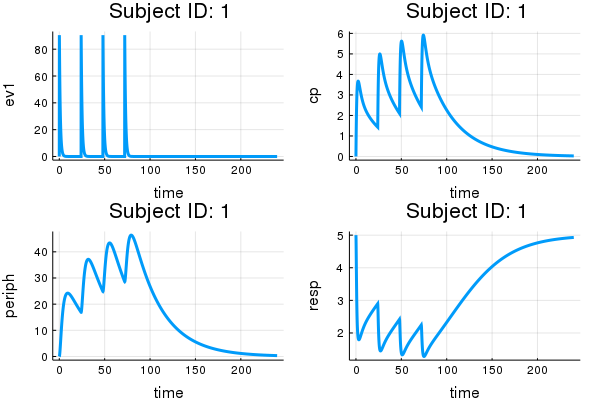
\includegraphics[width=8cm]{multiple-responses.png}
    \caption{Multiple Dosing Model Simulation Output}
    \label{fig:Pumas-mr}
\end{figure}

\begin{figure}
\begin{lstlisting}[mathescape=true]
@model begin
    @param   $\theta$ $\in$ VectorDomain(12)
    @random  $\eta$ $\sim$ MvNormal(Matrix{Float64}(I, 11, 11))

    @pre begin
        Ka1     = $\theta$[1]
        CL      = $\theta$[2]*exp($\eta$[1])
        Vc      = $\theta$[3]*exp($\eta$[2])
        Q       = $\theta$[4]*exp($\eta$[3])
        Vp      = $\theta$[5]*exp($\eta$[4])
        Kin     = $\theta$[6]*exp($\eta$[5])
        Kout    = $\theta$[7]*exp($\eta$[6])
        IC50    = $\theta$[8]*exp($\eta$[7])
        IMAX    = $\theta$[9]*exp($\eta$[8])
        $\gamma$        = $\theta$[10]*exp($\eta$[9])
        Vmax    = $\theta$[11]*exp($\eta$[10])
        Km      = $\theta$[12]*exp($\eta$[11])
    end

    @init begin
        Resp = $\theta$[6]/$\theta$[7]
    end

    @dynamics begin
        Ev1'    = -Ka1*Ev1
        Cent'   =  Ka1*Ev1 - (CL+Vmax/(Km+(Cent/Vc))+Q)*(Cent/Vc)  
                 + Q*(Periph/Vp)
        Periph' =  Q*(Cent/Vc) - Q*(Periph/Vp)
        Resp'   =  Kin*(1-(IMAX*(Cent/Vc)^$\gamma$/(IC50^$\gamma$+(Cent/Vc)^$\gamma$)))  
                 - Kout*Resp
    end

    @derived begin
        ev1    = Ev1
        cp     = Cent / $\theta$[3]
        periph = Periph
        resp   = Resp
    end
end
\end{lstlisting}
\caption{Pumas Multiple Response Model}
\label{code:Pumas}
\end{figure}

This Julia macro was developed by parsing the user's dynamical expression into the ModelingToolkit.jl IR. By doing so, Pumas.jl utilizes ModelingToolkit.jl's compilation pathway to generate Julia functions for the differential equation solvers. Additionally, Pumas can utilize this pathway to generate expressions for the analytic computation of Jacobians and sensitivity equations. These sensitivity equations of a differential equation are an extension of the ODEs which compute the derivative of the solution with respect to the parameters. These equations are given by:

\begin{equation}
\frac{d}{dt}\left(\frac{\partial u}{\partial p_{i}}\right)=\frac{\partial f}{\partial u}\frac{\partial u}{\partial p_{i}}+\frac{\partial f}{\partial p_{i}}\label{eq:clsa}
\end{equation}
where $\frac{\partial f}{\partial u}$ is the Jacobian of the derivative
function $f$ with respect to the current state, and $\frac{\partial f}{\partial p_{i}}$ is the gradient of the derivative function with respect to the $i$th
parameter. These sensitivity equations thus give the gradient of the solution with respect to the differential equation parameters which is then utilized by parameter optimization schemes such as BFGS from Optim.jl \cite{mogensen2018optim} when trying to estimate $\theta$ and $\eta$ from clinical trial data  \cite{sommer_numerical_nodate}. Crucially, the authors of Pumas.jl do not need to create the code for handling such symbolic calculations in their DSL since, by targeting ModelingToolkit.jl IR, these transformations exist as part of a common toolkit. A secondary effect of this modularization is that the Pumas.jl authors contribute these types of symbolic transformations to ModelingToolkit.jl's open source repository, which in turn allows the same techniques to be utilized by the DSLs of other packages.

\section{Future Work \label{sec:future}}

Continued development of ModelingToolkit.jl is focusing on expanding the feature set and incorporating ModelingToolkit into more DSLs. In our current form, the equations for systems of delay, stochastic, and differential-algebraic differential equations are representable but are lacking a system type. Our short term goals include added \texttt{AbstractSystem} types and compilation processes for these systems. Once these systems have a canonical representation, our existing symbolic transformations can be utilized to implement transformations such as DAE index reduction and computing analytical Jacobians of delay differential equation systems. With this litany of differential equation systems, we are looking into creating a higher level \texttt{ODESystem} which inspects the system's definition and auto-classifies the resulting equations. This would allow Pumas.jl to support these additional types of models without modification.

Feedback from the Julia community has signaled that one important avenue for this DSL is in developing and supporting large complex models. Along these lines, the detection of construction of analytical forms for sparse Jacobians is a natural extension of current functionality that is being investigated. Additionally, we are looking to introduce a new \texttt{Component} primitive which itself is a system that can be embedded within a system. For example, a \texttt{Heart} component would be a system of ODEs describing the chemical reactions of the heart, while a \texttt{Gut} component describes the chemical reactions of the gut, and from those two components we would construct a system of differential equations which incorporates these two parts and allows for interactions. This modularization would allow Modelica-type models to be represented within ModelingToolkit.

One final short term goal is to incorporate ModelingToolkit into the DiffEqBiological.jl reaction network DSL. Currently the arrow syntax of the chemical reaction expressions are parsed and a multi-stage process builds Julia expressions which are then transformed into SymEngine \cite{symengine} expressions in order to perform the required symbolic transformations and Jacobian calcluations, and a compilation toolchain then converts the resulting SymEngine expressions into Julia functions for DifferentialEquations.jl. A quick way to do the integration would be to intercept the process at the transformation to SymEngine expressions, instead building ModelingToolkit \texttt{Expression}s. Down the line, we would like to investigate whether the chemical reactions themselves could be represented within ModelingToolkit IR, so that transformation and analysis on the chemical reaction level could take place within this system.

\section{Acknowledgments}

We would like to acknowledge Julia Computing and the University of Maryland Baltimore's Center for Translational Medicine for sponsoring the development of Pumas and ModelingToolkit. Additionally, we graciously thank individual contributors to both projects.

\section{Resources}

ModelingToolkit.jl is available on GitHub under the MIT ``Expat'' License: \url{https://github.com/JuliaDiffEq/ModelingToolkit.jl}. Pumas.jl is available
at \url{https://github.com/PumasAI/Pumas.jl}

% **************GENERATED FILE, DO NOT EDIT**************

\bibliographystyle{juliacon}
\bibliography{ref.bib}


\end{document}

% Inspired by the International Journal of Computer Applications template
